\subsection{Smart Contracts}
\label{subsec:02_smart_contracts}

This section looks at the concept of smart contracts on the example of Ethereum.
Ethereum is a blockchain ''with built-in programming language'', or in other words a ''consensus-based globally executed virtual machine''.
The Ethereum project started in 2015 and has gained popularity since then. It is second place in terms of market capitalization according to coinmarketcap.com, right after bitcoin and followed by ripple \cite{coinmarketcap}.

Nodes in the Ethereum network make up the Ethereum Virtual Machine (EVM). Smart contracts are written in the programming language solidity. They get compiled to bytecode that the EVM can understand.
Once deployed on the blockchain, the code cannot be changed. Deploying smart contracts means mining them into the blockchain, thus deploying smart contracts costs a fee like every other transaction. Once they are there, they are part of the blockchain history. Every smart contract on the blockchain lives at an address where the contracts exposed functions and variables can interact with. Smart contracts can inherit from smart contracts and interact with other smart contracts.

Smart contracts can also be sent the cryptocurrency ether to. Sending ether to a smart contract that does not provide functionality to retrieve those ethers means they are lost forever in the contract. This is crucial especially when designing contracts that implement business logic or any contracts for that matter. Smart contracts should be reviewed and audited carefully and tested for vulnerabilities else its weaknesses can be exploited like in the infamous ``DAOgi`` attack.

Every transaction on the Ethereum blockchain costs a fee called gas. Gas is expressed in ether. The miner that mines a transaction collects the gas associated with it, thus gas serves as an incentive for miners to mine and contribute to the network. There is a defined set of operations with their respective gas costs in the Ethereum yellow paper \cite{ethereumyellowpaer}.
Figure \ref{fig:smart_contract_fees} shows and excerpt of those costs.

\begin{figure}[ht!]
  \begin{center}
    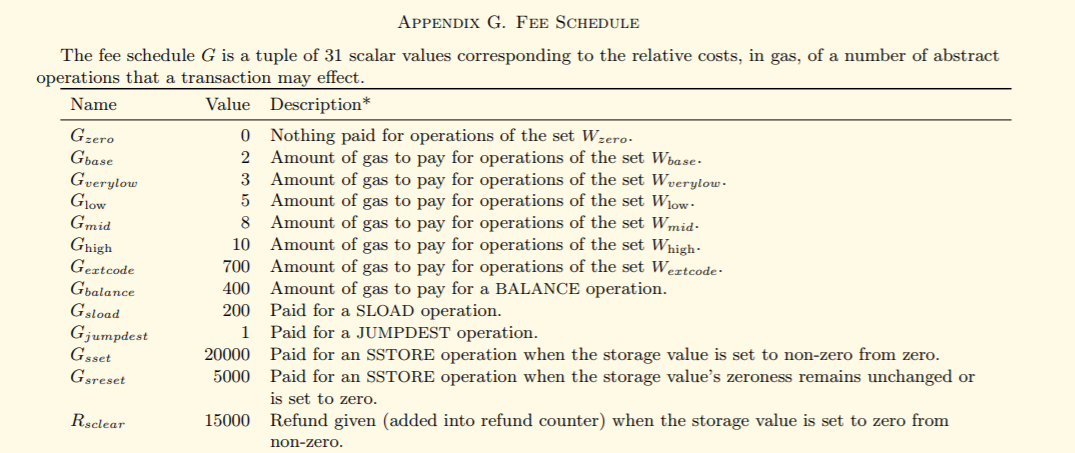
\includegraphics[scale=0.6]{Talk7/img/smart_contracts/gas-fees}
  \end{center}
  \caption{Smart contract fees as shown in the ethereum yellow paper}
  \label{fig:smart_contract_fees}
\end{figure}

Miners generally prioritize transactions with a higher potential gain (gas). The total gas fee to be paid is calculated by the gas price times the amount of gas to use. If the gas price for a transaction is set high, the transaction is mined to the blockchain faster. If on the other hand the price is set low, miners choose to mine other transactions first before mining transactions with a lower price. How high the gas price is is determined by the market. During peak network traffic, gas prices are high because as more people want their transaction to go through. Contrarily, prices drop when the network is more relaxed.

A transaction has a gas limit that can be set. This is to indicate the maximum amount of gas a transaction can use up before it is aborted. The gas limit times the gas price is the maximum amount the issuer is willing to pay for a transaction. In case of an endless loop, the execution will only last until the gas limit is used up.
If the gas limit is too little, the computation will run out of gas before it is finished, it will be reverted, and the gas paid will be lost. If the gas limit is higher than the amount of gas used, the remaining gas will be refunded to the sender of the transaction.

Miners can only put so many transactions in a block that block gas limit is not exceeded. This is also not a fixed value as miners can vote with each block to increase or decrease the block gas limit by a certain amount. Block gas limit serves to keep propagation of blocks and transaction time low by essentially limiting the size of the blocks.

The following overview sums up the key terms as mentioned above \cite{blockgeeks}:
\begin{itemize}
  \item {\textbf{gas}: How much gas a transaction needs }
  \item {\textbf{gas prize}: How much ether a unit of gas costs, determined by the market}
  \item {\textbf{gas limit}: Maximum amount of gas to use up for a transaction}
  \item {\textbf{transaction fee}: Gas used times gas price}
  \item {\textbf{block gas limit}: Maximum sum of gas of all transactions in a block}

\end{itemize}

In fact, not all smart contract interactions cost gas. Functions that do not modify the state of a contract, and hence the blockchain, do not need to be mined by a miner.
Calling those functions will still use gas, because every operation in the EVM uses gas, but that gas is refunded immediately as calling those functions does not result in a transaction.
In solidity those functions have the modifier ``pure'' or ``view''. Functions denoted with ``pure'' don't even read state variables. Both those functions can be run on a single node in the EVM and
nothing has to be propagated to the network thus no transaction has to be mined into the blockchain and no gas fee has to be paid\cite{blockgeeks}.

\begin{lstlisting}[language=Solidity,caption={Smart contract example},,label={solidity_example}]
  pragma solidity 0.5.0;

  contract MyContract {

    string private myString = "foo";

    function getString() view returns (string) {
        return myString;
    }

    function setString (string _string) {
        myString = _string;
    }
  }
  \end{lstlisting}

In the smart contract example \ref{solidity_example}, the functions ``setString'' modifies the state, namely the variable ``myString'', thus a transaction needs to be recorded in the blockchain and gas has to be paid.
The function ``getString'' on the other hand is denoted with the keyword ``view'', no state variables are modified so no transactions are required and no gas fee has to be paid.

Smart contracts allow programming on the blockchain which opens up a multitude of possibilities also in the context of cyber security for which upcoming sections discuss some solutions.
